\documentclass[aspectratio=169]{beamer}
\usetheme{SimplePlus}

\usepackage{tikz}
\usepackage{pgfplots}
\pgfplotsset{compat=1.17}
\usepackage{mathtools}
\usepackage{centernot}
\usepackage{amsmath, amssymb, amsthm, bm}
\DeclareMathOperator{\grad}{\nabla}
\renewcommand{\P}{\mathbb{P}}
\newcommand{\R}{\mathbb{R}}
\newcommand{\ttag}[1]{(#1)}

\title{Some things we did not study}
\author{Nicol\'as A. Barnafi}
\date{}

\begin{document}

\begin{frame}
    \titlepage
\end{frame}

\begin{frame}{The Limits of Lax-Milgram}
    Throughout this course, we have relied heavily on the \textbf{Lax-Milgram lemma} and the assumption of \textbf{ellipticity}.

    \vspace{0.3cm}
    However, many critical physical models break this assumption. In this final lecture, we provide a roadmap for the mathematical machinery required to analyze problems involving:
    \begin{itemize}
        \item Loss of coercivity (Compact perturbations).
        \item Constraints and Lagrange multipliers (Saddle point problems).
        \item Nonlinear material laws and advection (Nonlinear analysis).
        \item Evolution in time (Bochner spaces).
        \item PDE-constrained optimization (Optimal control).
    \end{itemize}
\end{frame}

\section{Compact Perturbations}
\begin{frame}{1. Compact Perturbations \& Fredholm Theory}
    \textbf{Motivation:} High-frequency wave propagation, such as the Helmholtz equation $-\Delta u - k^2 u = f$. The sign of the $k^2$ term destroys coercivity.

    \vspace{0.2cm}
    \textbf{The Abstraction:}
    We analyze operators of the form $A - K$, where $A: V \to V'$ is an elliptic isomorphism and $K: V \to V'$ is a \textbf{compact operator}. The bilinear form satisfies a \textit{G\r{a}rding inequality}:
    $$ a(v, v) \ge \alpha \|v\|_V^2 - C \|v\|_H^2 \quad \text{where } V \hookrightarrow\hookrightarrow H $$

    \vspace{0.2cm}
    \textbf{Analytical Toolkit:}
    \begin{itemize}
        \item \textbf{Fredholm Alternative:} For such operators, injectivity $\iff$ surjectivity.
        \item Well-posedness reduces to proving that $u=0$ is the \textit{only} solution to the homogeneous problem (often requiring physical radiation conditions).
    \end{itemize}
\end{frame}

\section{Saddle Point Problems}
\begin{frame}{2. Saddle Point Problems}
    \begin{columns}
        \begin{column}{0.6\textwidth}
            \textbf{Motivation:} Incompressible fluid flow (Stokes) or mixed formulations (Darcy). We must minimize an energy functional subject to a hard constraint (e.g., $\text{div } u = 0$).
            
            \vspace{0.2cm}
            \textbf{The Abstraction:}
            Introducing a Lagrange multiplier $p$ leads to a block-matrix system:
            $$ \begin{pmatrix} A & B^* \\ B & 0 \end{pmatrix} \begin{pmatrix} u \\ p \end{pmatrix} = \begin{pmatrix} f \\ g \end{pmatrix} $$
            
            \vspace{0.2cm}
            \textbf{Analytical Toolkit:}
            \begin{itemize}
                \item \textbf{LBB Theory:} Well-posedness hinges on the \textit{Ladyzhenskaya-Babu\v{s}ka-Brezzi (inf-sup) condition} for the constraint operator $B$.
                \item $\inf_{q \in Q} \sup_{v \in V} \frac{b(v,q)}{\|v\|_V \|q\|_Q} \ge \beta > 0$.
            \end{itemize}
        \end{column}
        \begin{column}{0.4\textwidth}
            \begin{center}
            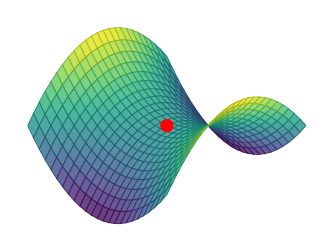
\begin{tikzpicture}[scale=0.8]
                \begin{axis}[
                    hide axis, colormap/viridis, 
                    view={45}{35}, width=6cm, height=6cm
                ]
                    \addplot3[surf, domain=-2:2, y domain=-2:2, opacity=0.8] {x^2 - y^2};
                    \fill[red] (axis cs:0,0,0) circle (3pt);
                \end{axis}
            \end{tikzpicture}
            \end{center}
        \end{column}
    \end{columns}
\end{frame}

\section{Nonlinear Problems}
\begin{frame}{3. Nonlinear Problems}
    \textbf{Motivation:} Large solid deformations, non-Newtonian fluids ($p$-Laplacian), or convective acceleration in Navier-Stokes. The mapping $u \mapsto A(u)$ is no longer linear.

    \vspace{0.2cm}
    \textbf{The Abstraction:}
    Find $u \in V$ such that $\langle A(u), v \rangle = \langle f, v \rangle \quad \forall v \in V$.

    \vspace{0.2cm}
    \textbf{Analytical Toolkit:}
    \begin{itemize}
        \item \textbf{Fixed Point Theorems:} (Banach, Brouwer, Schauder) Reformulate as $u = T(u)$ and use contractivity or compactness to find stationary points.
        \item \textbf{Monotone Operator Theory:} Generalizes positive-definiteness. 
        $$ \langle A(u) - A(v), u - v \rangle \ge 0 $$
        \item \textbf{Minty-Browder Theorem:} Guarantees existence and uniqueness for operators that are monotone, coercive, and hemicontinuous.
    \end{itemize}
\end{frame}

\section{Time-Dependent Problems}
\begin{frame}{4. Time-Dependent Problems (Evolution PDEs)}
    \textbf{Motivation:} Heat diffusion (parabolic) or wave propagation (hyperbolic). Space and time cannot be treated symmetrically.

    \vspace{0.2cm}
    \textbf{The Abstraction:}
    We map time to a functional space over the spatial domain. The solution $u(t)$ is a trajectory in a Banach space $V$.
    $$ \dot{u}(t) + Au(t) = f(t), \quad u(0) = u_0 $$

    \vspace{0.2cm}
    \textbf{Analytical Toolkit:}
    \begin{itemize}
        \item \textbf{Bochner Spaces:} $L^p(0,T; V)$, requiring rigorous definitions of integration for space-valued functions.
        \item \textbf{Faedo-Galerkin Method:} Prove well-posedness by passing to the limit on a sequence of finite-dimensional ODE systems.
    \end{itemize}
\end{frame}

\section{Optimal Control}
\begin{frame}{5. Optimal Control (PDE-Constrained Optimization)}
    \textbf{Motivation:} Engineering design. Finding the optimal boundary heating to achieve a desired internal temperature, or optimizing aerodynamic shape to minimize drag.

    \vspace{0.2cm}
    \textbf{The Abstraction:}
    Minimize a cost functional $J(u, z)$ with respect to a state $u$ and control $z$, subject to the state constraint $E(u, z) = 0$ (the PDE).

    \begin{center}
    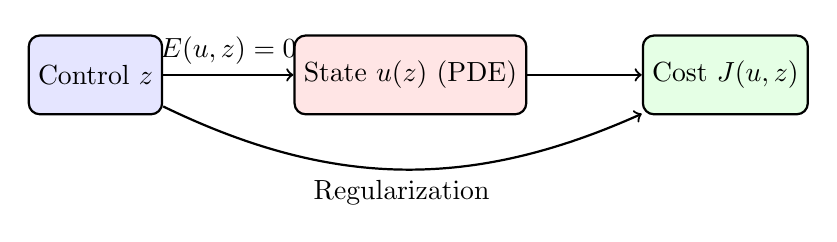
\begin{tikzpicture}[node distance=2.5cm, auto, thick]
        \node[draw, rectangle, fill=blue!10, rounded corners, minimum height=1cm] (control) {Control $z$};
        \node[draw, rectangle, fill=red!10, rounded corners, right of=control, node distance=4cm, minimum height=1cm] (state) {State $u(z)$ (PDE)};
        \node[draw, rectangle, fill=green!10, rounded corners, right of=state, node distance=4cm, minimum height=1cm] (cost) {Cost $J(u,z)$};
        
        \draw[->] (control) -- node[above] {$E(u,z)=0$} (state);
        \draw[->] (state) -- (cost);
        \draw[->] (control) to[bend right=25] node[below] {Regularization} (cost);
    \end{tikzpicture}
    \end{center}

    \vspace{0.1cm}
    \textbf{Analytical Toolkit:}
    \begin{itemize}
        \item \textbf{Lagrangians \& Adjoints:} Define an adjoint PDE to compute the functional gradient efficiently ($\nabla_z J$). KKT conditions in infinite dimensions.
    \end{itemize}
\end{frame}

\begin{frame}
    \titlepage
\end{frame}

\end{document}
